% !TeX spellcheck = pl_PL
\documentclass[a4paper]{article}
\usepackage{polski}
\usepackage[utf8]{inputenc}
\usepackage{lmodern}
\usepackage{indentfirst}
\usepackage{graphicx}
\usepackage{amsmath}
\usepackage[unicode, bookmarks=true]{hyperref} %do zakładek
\usepackage{tabto} % do tabulacji
\NumTabs{6} % globalne ustawienie wielkosci tabulacji
\usepackage{array}
\usepackage{multirow}
\usepackage{listings}
\usepackage{array}
\usepackage{dcolumn}
\usepackage{bigstrut}
\usepackage{color}
\usepackage{epigraph}
\usepackage{wrapfig}
\usepackage{MnSymbol}
\usepackage{xparse}
\usepackage[usenames,dvipsnames]{xcolor}
\usepackage[T1]{fontenc}
\usepackage{enumitem}
\usepackage{courier}
\usepackage[toc,page]{appendix}
\usepackage{subfigure}

\lstset{basicstyle=\footnotesize\ttfamily,breaklines=true}
\lstset{framextopmargin=50pt,frame=leftline}

%załączniki - polskie nazwy 
\renewcommand\appendixtocname{Załącznik} %spis treści 
\renewcommand\appendixpagename{Załącznik} %strona sekcji 

\makeatletter
\newcommand*{\rom}[1]{\expandafter\@slowromancap\romannumeral #1@}
\makeatother

\setlength{\epigraphwidth}{0.5\textwidth}

\newcommand{\HRule}{\rule{\linewidth}{0.5mm}}
\setlength{\textheight}{24cm}
\setlength{\textwidth}{15.92cm}
\setlength{\footskip}{10mm}
\setlength{\oddsidemargin}{0mm}
\setlength{\evensidemargin}{0mm}
\setlength{\topmargin}{0mm}
\setlength{\headsep}{10mm}
\setlength{\voffset}{-7mm}

\makeatletter
\def\@seccntformat#1{%
	\expandafter\ifx\csname c@#1\endcsname\c@section
	\thesection.
	\else
	\csname the#1\endcsname\quad
	\fi}
\makeatother

%\titlespacing*{\section}
%{0pt}{0pt}{-0.2cm}

\usepackage{fancyhdr} % Required for modifying headers and footers
\fancyhead[L]{\textsf{\rightmark}} % Top left header
\fancyhead[R]{\textsf{\leftmark}} % Top right header
\renewcommand{\headrulewidth}{1.2pt} % Rule under the header
\fancyfoot[C]{\textbf{\textsf{\thepage}}} % Bottom center footer
\renewcommand{\footrulewidth}{1.2pt} % Rule under the footer
\pagestyle{fancy} % Use the custom headers and footers throughout the document

\usepackage{titlesec}
\makeatletter
\@addtoreset{section}{part}
\makeatother

\titleformat{\paragraph}
{\normalfont\normalsize\bfseries}{\theparagraph}{1em}{}
\titlespacing*{\paragraph}
{0pt}{3.25ex plus 1ex minus .2ex}{1.5ex plus .2ex}

\begin{document}
	%\kslistofremarks
	%	\maketitle
	% !TeX spellcheck = pl_PL
\begin{titlepage}
	\begin{center}
		
		% Upper part of the page. The '~' is needed because \\
		% only works if a paragraph has started.
		
\includegraphics[width=0.5\textwidth]{logo.png}~\\[1cm]
		%?[width=0.15\textwidth]
		
		\textsc{\LARGE Politechnika Śląska w Gliwicach}\\[1.5cm]
		
		\textsc{\Large Algorytmy Kompresji Danych}\\
		\textsc{\today}\\[0.5cm]
		
		% Title
		\HRule \\[0.4cm]
		{ \huge \bfseries Porównanie PNG, JPEG-LS i JPEG2000 w kompresji bezstratnej \\[0.4cm] }
		
		\HRule \\[1.5cm]
		
		% Author and supervisor
		\textsc{\Large Autor:} \\
		Bartłomiej Buchała \\
		[1.0cm]
		Informatyka SSM, semestr II \\
		Rok akademicki 2016/2017 \\
		Grupa OS1
		
		\vfill

	\vfill
\end{center}
\end{titlepage}
	
	\tableofcontents
	\newpage
	\section{Wstęp}

Cel projektu: przeprowadzić porównanie algorymtów PNG, JPEG-LS i JPEG2000 w trybie kompresji bezstratnej. Porównywane implementacje ocenić pod względem:

\begin{itemize}
	\item Uzyskiwanych współczynników,
	\item Prędkości kompresji.
\end{itemize}

Należy przeprowadzić badania dla barwnych i czarno-białych obrazów. W tym celu posłużono się obrazami z zestawu Waterloo (\url{http://links.uwaterloo.ca/Repository.html}):

\begin{itemize}
	\item Waterloo Greyscale 2 (obrazy w odcieniach szarości)
	\item Waterloo Colour Set (obrazy barwne)
\end{itemize}
	
	\section{Użyte algorytmy}

\subsection{PNG}

\textbf{PNG} (ang. \textit{Portable Network Graphics}) -- to rastrowy format plików graficznych oraz system bezstratnej kompresji obrazów barwnych oraz w odcieniach szarości. Został opracowany w 1995 roku jako następca formatu GIF.
Cechy algorytmu PNG:

\begin{itemize}
	\item Kompresor PNG jest schematem predykcyjnym.
	\item Kompresja polega na wykonaniu transformacji każdej linii obrazu, po czym skompresowaniu go za pomocą algorytmu deflate.
	\item Transformacja polega na obliczeniu różnicy pomiędzy wartością piksela, a wartością obliczoną na podstawie funkcji przewidującej.
	\item Funkcje przewidujące to funkcje wyliczające wartości na podstawie wartości sąsiadujących pikseli.
	\item Stosowane jest kodowanie LZ77, a do kodowania położenia i długości dopasowanej sekwencji używa sie kodów przedrostkowych zmiennej długości (predefiniowanych lub kodów Huffmana z ograniczeniem).
\end{itemize}

\subsection{JPEG-LS}

\textbf{JPEG-LS} jest nowym standardem komitetu JPEG dla kompresji bezstratnej obrazów wynalezionym w 1999 roku. Jest następcą Lossless JPG opartym o algorytm LOCO-I. Wykorzystywany jest ze względu na osiągane współczynniki kompresji (bliskie najlepszym) oraz dużą elastyczność umożliwiającą implementację rozszerzeń. Oprócz tego istnieje ,,prawie bezstratny'' (ang. \textit{nearly lossless}) wariant tego algorytmu.

Uogólniony schemat algorytmu JPEG-LS:

\begin{enumerate}
	\item \textbf{Wykrywanie krawędzi pionowych i poziomych} -- stosowany w tym celu jest prosty predykat nieliniowy (wyznaczanie jedynie przy pomocy stałopozycyjnych operacji dodawania/odejmowania i porównań liczb stałopozycyjnych).
	\item \textbf{Kodowanie} -- przy pomocy kodera entropijnego i zmodyfikowanej (uproszczonej) rodziny kodów Rice'a. Na tym etapie koduje się również błędy predykcji.
	\item \textbf{Modelowanie kontekstu} -- wyznaczony na podstawie 3 gradientów model jest dedykowany dla kodów rodziny Rice'a.
\end{enumerate}

\subsection{JPEG2000}

\textbf{JPEG-2000} podobnie jak JPEG-LS jest następcą algorytmu JPEG wyłonionym w drodze konkursu. Opracowany w 2000 roku, stanowi standard komitetu JPEG zarówno dla stratnej, jak i bezstratnej kompresji obrazów. Jest algorytmem przeznaczonym dla obrazów barwnych i w odcieniach szarości opartym o transformatę falkową. Pozwala na kodowanie piramidowe i progresywne.

Uogólniony schemat algorytmu JPEG2000:

\begin{enumerate}
	\item \textbf{Sprowadzenie nominalnego zakresu jasności pikseli do przedziały symetrycznego względem 0} -- jest to krok tożsamy z tym wykonywanym w algorytmie JPEG.
	\item \textbf{Transformacja przestrzeni barw} -- może być nieodwracalna lub odwracalna. Ta pierwsza możliwa jest tylko razem z nieodwracalną transformatą falkową.
	\item \textbf{Podział składowej na kafelki} -- realizowany poprzez nałożenie siatki prostokątnej na obraz (najczęściej o wymiarach 256 na 256 pikseli). Krawędzie siatki nie muszą się pokrywać z krawędziami obrazu, a obraz może mieścić się w jednym kafelku.
	\item \textbf{Wyznaczenie transformaty falkowej dla każdego kafelka} -- przed transformatą należy ekstrapolować wiersze. W przypadku kompresji bezstratnej, stosujemy transformatę odwracalną.
	\item \textbf{Kwantyzacja współczynników transformaty} -- dla kompresji bezstratnej krok zawsze wynosi 1. W przypadku operacji kompresji stratnej koder dobiera krok, aby możliwe było osiągnięcie zadanego współczynnika.
	\item \textbf{Kodowanie skwantowanych współczynników} -- przy pomocy kodera arytmetycznego.
	\item \textbf{Zapisanie zakodowanych danych w pliku o strukturze opisej przez standard.}
\end{enumerate}
	
	\section{Wykorzystane biblioteki}

\subsection{PNG -- pnmtopng}

\subsubsection{Instalacja}

\textbf{pnmtopng} jest elementem pakietu NetPBM. Aby umożliwić korzystanie z biblioteki na systemie Unixowym, należy:

\begin{enumerate}
	\item Posiadać zainstalowane wymagane LibPNG, ZLIB, dowolny kompilator języka C oraz Perl w wersji 6.0 lub nowszy.
	\item Pobrać pliki źródłowe spakowane do formatu .tar ze strony SourceForge (\url{https://sourceforge.net/projects/netpbm/files/}).
	
	\item Wypakować pliki do wybranego przez siebie folderu.
	
	\item Wykonać komendy
	\begin{lstlisting}[language=bash]
	./configure
	make package
	./installnetpbm
	\end{lstlisting}
\end{enumerate}

W przypadku Windowsa, należy posłużyć środowiskami Cygwin lub Djgpp.

Prostszą alternatywą jest pobranie skompilowanych plików binarnych ze strony: \url{http://gnuwin32.sourceforge.net/packages/netpbm.htm}

\subsubsection{Uruchamianie}

Aby uruchomić kompresję plików, należy posłużyć się aplikacją \textbf{pnmtopng}. Przykładowe wywołanie programu w celu kompresji pliku \textit{clegg.pp\textsl{}m}:

\begin{lstlisting}[language=bash]
	pnmtopng clegg.pnm >clegg.png
\end{lstlisting}

\subsection{JPEG-LS -- SPMG/JPEG-LS}

\subsubsection{Instalacja}

\subsubsection{Uruchamianie}

\subsection{JPEG2000 -- JasPer}

\subsubsection{Instalacja}

\textbf{JasPer} jest otwarto źródłową biblioteką zawierającą implementację algorytmu JPEG2000. W celu instalacji na systemie Windows należy:

\begin{enumerate}
	\item Pobrać i wypakować pliki źródłowe ze strony projektu (\url{http://www.ece.uvic.ca/~frodo/jasper/}) do wybranej przez siebie lokalizacji.
	
	\item Utworzenie dodatkowy zmiennych środowiskowych:
	\begin{enumerate}
		\item \textbf{\%SOURCE\textunderscore DIR\%} -- katalog nadrzędny, w którym wypakowane zostały pobrane pliki
		\item \textbf{\%BUILD\textunderscore DIR\%} -- ścieżka do katalogu używanego do zbudowania aplikacji
		\item \textbf{\%INSTALL\textunderscore DIR\%} -- ścieżka do katalogu używanego do zainstalowania aplikacji
	\end{enumerate}
	Zmienne te są zdefiniowane pliku make i będą wykorzystywane w trakcie instalacji.
	
	\item W wierszy poleceń wykonać polecenie:
	
	\begin{lstlisting}[language=bash]
	cmake -help
	\end{lstlisting}
	
	Pozwala to podejrzeć nazwy wszystkich dostępnych generatorów (programów umożliwiających kompilację plików źródłowych).
	
	\item Za pomocą wybranego przez siebie generatora (parametr -G) wykonać komendę tworzącą plik solucji .sln.
	
	\begin{lstlisting}[language=bash]
	cmake -G "Visual Studio 14 2015 Win64" -H%SOURCE_DIR% -B%BUILD_DIR% ^ -DCMAKE_INSTALL_PREFIX=%INSTALL_DIR%
	\end{lstlisting}
	
	\item W wierszu poleceń programisty (ang. \textit{Developer Command Line}) wykonać komendę:
	
	\begin{lstlisting}[language=bash]
	msbuild %build_dir%\INSTALL.vcxproj
	\end{lstlisting}
	
	Spowoduje to utworzenie skompilowanego programu jasper.exe w ścieżce podanej w \%INSTALL\textunderscore DIR\%.
\end{enumerate}



\subsubsection{Uruchamianie}

Aby uruchomić program jasper.exe, należy w pierwszej kolejności skopiować do tego samego katalogu bibliotekę \textit{libjasper.dll}, wygenerowaną wcześniej w folderze \textit{lib}. Może również dojść do sytuacji, w jakiej nie zostanie wykryta biblioteka \textit{ucrtbased.dll}. W takim przypadku należy pobrać ją z internetu i wypakować ją w \textit{$C:\backslash Windows\backslash System32\backslash$}. Przykładowa komenda uruchamiająca kompresję (plik clegg.ppm):

\begin{lstlisting}[language=bash]
jasper.exe --input clegg.ppm --output clegg.jp2
\end{lstlisting}
	
	\section{Porównanie wyników}

\subsection{Platforma testowa}

Testy przeprowadzono na komputerze stancjonarnym o następującej specyfikacji:

\begin{itemize}
	\item System operacyjny -- Windows 10 Home 64-bit.
	\item Procesor -- Intel Core i5 4590, taktowanie 3.30GHz.
	\item Pamięć RAM -- 8 GB 2-Kanałowy DDR3, taktowanie 1600 MHz.
\end{itemize}

\subsection{Badane wartości}

Jakość kompresji określono za pomocą współczynnika kompresji, którego można przedstawić przy pomocy wzoru:
\[
CR = \frac{ Skompresowany Rozmiar }{ Nieskompresowany Rozmiar } 
\]

W tym przypadku, im niższa wartość tym lepszy algorytm. Współczynnik można również zapisać procentowo.

Drugą mierzoną wartością był czas kompresji obliczany w milisekundach.

\subsection{Obrazy barwne}

Podstawą dla obrazów barwnych był format \textbf{PPM} -- odmiana bitmapy, będącej formą zapisu grafiki rastrowej. PPM jest przeznaczony dla obrazów kolorowych i zawiera maksymalnie do 24 bitów na piksel w trybie binarnym (8 bitów na każdy kolor).

Dostęp do kolorowych obrazów w wersji oryginalnej i we wszystkich skompresowanych formatach można znaleźć pod adresem \url{https://1drv.ms/f/s!AgqzGFHuQrvMh6YsXffaWhGLWCa-qQ}.

\begin{table}[!h]
	\centering
	\caption{\textbf{Clegg}}
	\label{my-label}
	\begin{tabular}{|c|c|c|c|c|}                                             
		\hline
		& \textbf{Rozmiar przed} & \textbf{Rozmiar po} & \textbf{Wspł. kompresji} & \textbf{Czas {[}ms{]}} \\ \hline 
		\textbf{PNG}      &          \multicolumn{1}{c|}{\multirow{2}{*}{2099 KB}}             &      475 KB               &         22,62 \%                 &              216               \\\cline{3-5}
		\textbf{JPEG-LS}  &                        &        638  KB         &      30,39 \%                  &         58                 \\\cline{3-5}
		\textbf{JPEG2000} &                        &        1370 KB             &       65,25 \%                   &        273              \\ \hline
	\end{tabular}
\end{table}

\begin{table}[!h]
	\centering
	\caption{\textbf{Frymire}}
	\label{my-label}
	\begin{tabular}{|c|c|c|c|c|}                                             
		\hline
		& \textbf{Rozmiar przed} & \textbf{Rozmiar po} & \textbf{Wspł. kompresji} & \textbf{Czas {[}ms{]}} \\ \hline 
		\textbf{PNG}      &          \multicolumn{1}{c|}{\multirow{2}{*}{3620 KB}}             &         380 KB              &        10,49 \%                   &            176                 \\\cline{3-5}
		\textbf{JPEG-LS}  &                        &        914 KB             &         25,25 \%                 &           59               \\\cline{3-5}
		\textbf{JPEG2000} &                        &         1561 KB               &          43,11 \%                &       719               \\ \hline
	\end{tabular}
\end{table}

\begin{table}[!h]
	\centering
	\caption{\textbf{Lena3}}
	\label{my-label}
	\begin{tabular}{|c|c|c|c|c|}                                             
		\hline
		& \textbf{Rozmiar przed} & \textbf{Rozmiar po} & \textbf{Wspł. kompresji} & \textbf{Czas {[}ms{]}} \\ \hline 
		\textbf{PNG}      &          \multicolumn{1}{c|}{\multirow{2}{*}{769 KB}}             &      466 KB               &        60,54 \%                  &         103                    \\\cline{3-5}
		\textbf{JPEG-LS}  &                        &         436 KB            &      56,81 \%                   &         30                 \\\cline{3-5}
		\textbf{JPEG2000} &                        &     435 KB             &         57,93 \%                 &       440               \\ \hline
	\end{tabular}
\end{table}

\begin{table}[!h]
	\centering
	\caption{\textbf{Monarch}}
	\label{my-label}
	\begin{tabular}{|c|c|c|c|c|}                                             
		\hline
		& \textbf{Rozmiar przed} & \textbf{Rozmiar po} & \textbf{Wspł. kompresji} & \textbf{Czas {[}ms{]}} \\ \hline 
		\textbf{PNG}      &          \multicolumn{1}{c|}{\multirow{2}{*}{1153 KB}}             &      605 KB               &          52,44 \%                &            230                 \\\cline{3-5}
		\textbf{JPEG-LS}  &                        &       543 KB             &        46,94 \%                 &        44                  \\\cline{3-5}
		\textbf{JPEG2000} &                        &      432 KB               &        37,44 \%                 &       482               \\ \hline
	\end{tabular}
\end{table}

\begin{table}[!h]
	\centering
	\caption{\textbf{Peppers3}}
	\label{my-label}
	\begin{tabular}{|c|c|c|c|c|}                                             
		\hline
		& \textbf{Rozmiar przed} & \textbf{Rozmiar po} & \textbf{Wspł. kompresji} & \textbf{Czas {[}ms{]}} \\ \hline 
		\textbf{PNG}      &          \multicolumn{1}{c|}{\multirow{2}{*}{769 KB}}             &         418 KB            &        54,33 \%                  &         149                    \\\cline{3-5}
		\textbf{JPEG-LS}  &                        &          377 KB           &         49,01 \%                 &          29                \\\cline{3-5}
		\textbf{JPEG2000} &                        &        328 KB             &      42,64 \%                    &      367                \\ \hline
	\end{tabular}
\end{table}

\begin{table}[!h]
	\centering
	\caption{\textbf{Sail}}
	\label{my-label}
	\begin{tabular}{|c|c|c|c|c|}                                             
		\hline
		& \textbf{Rozmiar przed} & \textbf{Rozmiar po} & \textbf{Wspł. kompresji} & \textbf{Czas {[}ms{]}} \\ \hline 
		\textbf{PNG}      &          \multicolumn{1}{c|}{\multirow{2}{*}{1153 KB}}             &       792 KB              &         68,66 \%                 &           156                  \\\cline{3-5}
		\textbf{JPEG-LS}  &                        &        750  KB           &         64,93 \%                &          45                \\\cline{3-5}
		\textbf{JPEG2000} &                        &        512 KB             &      44,37 \%                   &      542                \\ \hline
	\end{tabular}
\end{table}

\begin{table}[!h]
	\centering
	\caption{\textbf{Serrano}}
	\label{my-label}
	\begin{tabular}{|c|c|c|c|c|}                                             
		\hline
		& \textbf{Rozmiar przed} & \textbf{Rozmiar po} & \textbf{Wspł. kompresji} & \textbf{Czas {[}ms{]}} \\ \hline 
		\textbf{PNG}      &          \multicolumn{1}{c|}{\multirow{2}{*}{1464 KB}}             &       155 KB              &            10,58 \%              &           95                  \\\cline{3-5}
		\textbf{JPEG-LS}  &                        &         287 KB            &      19,60 \%                   &          23                \\\cline{3-5}
		\textbf{JPEG2000} &                        &         624 KB            &         42,61 \%                 &       740               \\ \hline
	\end{tabular}
\end{table}

\begin{table}[!h]
	\centering
	\caption{\textbf{Tulips}}
	\label{my-label}
	\begin{tabular}{|c|c|c|c|c|}                                             
		\hline
		& \textbf{Rozmiar przed} & \textbf{Rozmiar po} & \textbf{Wspł. kompresji} & \textbf{Czas {[}ms{]}} \\ \hline 
		\textbf{PNG}      &          \multicolumn{1}{c|}{\multirow{2}{*}{1153 KB}}             &        667 KB             &      57,88 \%                   &          202                   \\\cline{3-5}
		\textbf{JPEG-LS}  &                        &      603  KB             &       52,35 \%                  &          46                \\\cline{3-5}
		\textbf{JPEG2000} &                        &      478 KB               &       41,46 \%                  &     547                 \\ \hline
	\end{tabular}
\end{table}




\begin{figure}[!h]
	\centering
	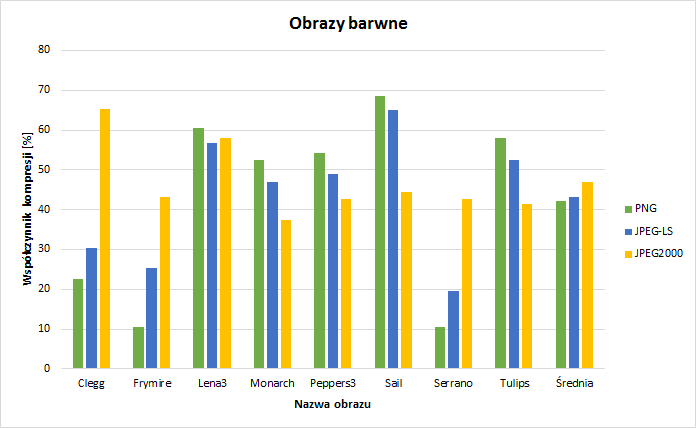
\includegraphics[width=1.1\textwidth]{./color.png}
	\caption{Wykres słupkowy dla obrazów kolorowych}
	\label{img:color}
\end{figure}

\clearpage








\subsection{Obrazy czarno-białe}

Podstawą dla obrazów z zestawu Waterloo Greyset 2 był format \textbf{PGM} -- odmiana bitmapy, będącej formą zapisu grafiki rastrowej. PGM jest przeznaczony dla w obrazów odcieniach szarości i zawiera 8 bitów na piksel.

Dostęp do czarno-białych obrazów w wersji oryginalnej i we wszystkich skompresowanych formatach można znaleźć pod adresem \url{https://1drv.ms/f/s!AgqzGFHuQrvMh6Yrr6Nukb3bG8dq6A}.

\begin{table}[!h]
	\centering
	\caption{\textbf{Barb}}
	\label{my-label}
	\begin{tabular}{|c|c|c|c|c|}                                             
		\hline
		& \textbf{Rozmiar przed} & \textbf{Rozmiar po} & \textbf{Wspł. kompresji} & \textbf{Czas {[}ms{]}} \\ \hline 
		\textbf{PNG}      &          \multicolumn{1}{c|}{\multirow{2}{*}{257 KB}}             &      170 KB               &    66,28 \%                     &           58                  \\\cline{3-5}
		\textbf{JPEG-LS}  &                        &       152 KB              &        59,17 \%                 &        10                  \\\cline{3-5}
		\textbf{JPEG2000} &                        &     150 KB                &        58,24 \%                 &        155              \\ \hline
	\end{tabular}
\end{table}

\begin{table}[!h]
	\centering
	\caption{\textbf{Boat}}
	\label{my-label}
	\begin{tabular}{|c|c|c|c|c|}                                             
		\hline
		& \textbf{Rozmiar przed} & \textbf{Rozmiar po} & \textbf{Wspł. kompresji} & \textbf{Czas {[}ms{]}} \\ \hline 
		\textbf{PNG}      &          \multicolumn{1}{c|}{\multirow{2}{*}{257 KB}}             &       149 KB              &      57,94 \%                    &           67                  \\\cline{3-5}
		\textbf{JPEG-LS}  &                        &       136 KB              &         53,19 \%                &         10                 \\\cline{3-5}
		\textbf{JPEG2000} &                        &      141 KB               &        55,07 \%                &        151              \\ \hline
	\end{tabular}
\end{table}

\begin{table}[!h]
	\centering
	\caption{\textbf{France}}
	\label{my-label}
	\begin{tabular}{|c|c|c|c|c|}                                             
		\hline
		& \textbf{Rozmiar przed} & \textbf{Rozmiar po} & \textbf{Wspł. kompresji} & \textbf{Czas {[}ms{]}} \\ \hline 
		\textbf{PNG}      &          \multicolumn{1}{c|}{\multirow{2}{*}{326 KB}}             &     18  KB              &    5,27 \%                     &            40                 \\\cline{3-5}
		\textbf{JPEG-LS}  &                        &        58 KB             &       17,63 \%                  &          5                \\\cline{3-5}
		\textbf{JPEG2000} &                        &     83 KB                &      25,25 \%                   &         142             \\ \hline
	\end{tabular}
\end{table}

\begin{table}[!h]
	\centering
	\caption{\textbf{Frog}}
	\label{my-label}
	\begin{tabular}{|c|c|c|c|c|}                                             
		\hline
		& \textbf{Rozmiar przed} & \textbf{Rozmiar po} & \textbf{Wspł. kompresji} & \textbf{Czas {[}ms{]}} \\ \hline 
		\textbf{PNG}      &          \multicolumn{1}{c|}{\multirow{2}{*}{303 KB}}             &        227 KB             &    75,01 \%                     &           57                  \\\cline{3-5}
		\textbf{JPEG-LS}  &                        &      229 KB               &       75,75 \%                  &         12                 \\\cline{3-5}
		\textbf{JPEG2000} &                        &      237 KB               &       78,22 \%                  &      125                \\ \hline
	\end{tabular}
\end{table}

\begin{table}[!h]
	\centering
	\caption{\textbf{Goldhill2}}
	\label{my-label}
	\begin{tabular}{|c|c|c|c|c|}                                             
		\hline
		& \textbf{Rozmiar przed} & \textbf{Rozmiar po} & \textbf{Wspł. kompresji} & \textbf{Czas {[}ms{]}} \\ \hline 
		\textbf{PNG}      &          \multicolumn{1}{c|}{\multirow{2}{*}{257 KB}}             &        157 KB             &      61,08 \%                   &               54              \\\cline{3-5}
		\textbf{JPEG-LS}  &                        &       151 KB              &         58,82 \%                &            10              \\\cline{3-5}
		\textbf{JPEG2000} &                        &       155 KB              &         60,47 \%                &       171               \\ \hline
	\end{tabular}
\end{table}

\begin{table}[!h]
	\centering
	\caption{\textbf{Lena2}}
	\label{my-label}
	\begin{tabular}{|c|c|c|c|c|}                                             
		\hline
		& \textbf{Rozmiar przed} & \textbf{Rozmiar po} & \textbf{Wspł. kompresji} & \textbf{Czas {[}ms{]}} \\ \hline 
		\textbf{PNG}      &          \multicolumn{1}{c|}{\multirow{2}{*}{257 KB}}             &      148 KB               &       57,57 \%                  &           63                   \\\cline{3-5}
		\textbf{JPEG-LS}  &                        &        136 KB             &         52,95 \%                &       10                   \\\cline{3-5}
		\textbf{JPEG2000} &                        &      139 KB               &          53,95 \%               &       150               \\ \hline
	\end{tabular}
\end{table}

\begin{table}[!h]
	\centering
	\caption{\textbf{Library}}
	\label{my-label}
	\begin{tabular}{|c|c|c|c|c|}                                             
		\hline
		& \textbf{Rozmiar przed} & \textbf{Rozmiar po} & \textbf{Wspł. kompresji} & \textbf{Czas {[}ms{]}} \\ \hline 
		\textbf{PNG}      &          \multicolumn{1}{c|}{\multirow{2}{*}{160 KB}}             &      103 KB               &    64,18 \%                     &           37                  \\\cline{3-5}
		\textbf{JPEG-LS}  &                        &     102 KB                &        63,69 \%                 &           6               \\\cline{3-5}
		\textbf{JPEG2000} &                        &     114 KB                &        71,20 \%                 &        127              \\ \hline
	\end{tabular}
\end{table}

\begin{table}[!h]
	\centering
	\caption{\textbf{Mandrill}}
	\label{my-label}
	\begin{tabular}{|c|c|c|c|c|}                                             
		\hline
		& \textbf{Rozmiar przed} & \textbf{Rozmiar po} & \textbf{Wspł. kompresji} & \textbf{Czas {[}ms{]}} \\ \hline 
		\textbf{PNG}      &          \multicolumn{1}{c|}{\multirow{2}{*}{257 KB}}             &     200 KB                &        76,28 \%                 &         49                    \\\cline{3-5}
		\textbf{JPEG-LS}  &                        &       194 KB             &        75,18 \%                &           10               \\\cline{3-5}
		\textbf{JPEG2000} &                        &       196 KB              &          76,37 \%               &     182                 \\ \hline
	\end{tabular}
\end{table}

\begin{table}[!h]
	\centering
	\caption{\textbf{Mountain}}
	\label{my-label}
	\begin{tabular}{|c|c|c|c|c|}                                             
		\hline
		& \textbf{Rozmiar przed} & \textbf{Rozmiar po} & \textbf{Wspł. kompresji} & \textbf{Czas {[}ms{]}} \\ \hline 
		\textbf{PNG}      &          \multicolumn{1}{c|}{\multirow{2}{*}{301 KB}}             &       248 KB              &      82,53 \%                   &            65                 \\\cline{3-5}
		\textbf{JPEG-LS}  &                        &       240 KB              &          80,64 \%               &            12              \\\cline{3-5}
		\textbf{JPEG2000} &                        &       252 KB              &          83,76 \%               &       241               \\ \hline
	\end{tabular}
\end{table}

\begin{table}[!h]
	\centering
	\caption{\textbf{Peppers2}}
	\label{my-label}
	\begin{tabular}{|c|c|c|c|c|}                                             
		\hline
		& \textbf{Rozmiar przed} & \textbf{Rozmiar po} & \textbf{Wspł. kompresji} & \textbf{Czas {[}ms{]}} \\ \hline 
		\textbf{PNG}      &          \multicolumn{1}{c|}{\multirow{2}{*}{257 KB}}             &      156 KB               &     60,56 \%                    &          56                   \\\cline{3-5}
		\textbf{JPEG-LS}  &                        &       144 KB              &       56,17 \%                  &             11             \\\cline{3-5}
		\textbf{JPEG2000} &                        &       148 KB              &       57,73 \%                  &        150              \\ \hline
	\end{tabular}
\end{table}

\begin{table}[!h]
	\centering
	\caption{\textbf{Washsat}}
	\label{my-label}
	\begin{tabular}{|c|c|c|c|c|}                                             
		\hline
		& \textbf{Rozmiar przed} & \textbf{Rozmiar po} & \textbf{Wspł. kompresji} & \textbf{Czas {[}ms{]}} \\ \hline 
		\textbf{PNG}      &          \multicolumn{1}{c|}{\multirow{2}{*}{257 KB}}             &         104 KB            &     40,35 \%                    &          88                   \\\cline{3-5}
		\textbf{JPEG-LS}  &                        &      133 KB               &          51,54 \%               &           9               \\\cline{3-5}
		\textbf{JPEG2000} &                        &      142 KB               &          55,39 \%               &     169                 \\ \hline
	\end{tabular}
\end{table}

\begin{table}[!h]
	\centering
	\caption{\textbf{Zelda}}
	\label{my-label}
	\begin{tabular}{|c|c|c|c|c|}                                             
		\hline
		& \textbf{Rozmiar przed} & \textbf{Rozmiar po} & \textbf{Wspł. kompresji} & \textbf{Czas {[}ms{]}} \\ \hline 
		\textbf{PNG}      &          \multicolumn{1}{c|}{\multirow{2}{*}{257 KB}}             &      137 KB               &     53,17 \%                    &          63                   \\\cline{3-5}
		\textbf{JPEG-LS}  &                        &      129 KB               &       50,17 \%                  &         9                 \\\cline{3-5}
		\textbf{JPEG2000} &                        &      128 KB               &       49,90 \%                  &        147              \\ \hline
	\end{tabular}
\end{table}


\begin{figure}[!h]
	\centering
	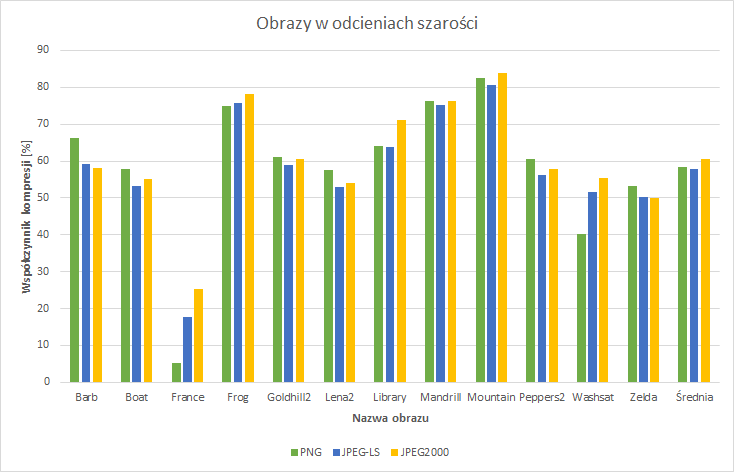
\includegraphics[width=1.1\textwidth]{./greyset.png}
	\caption{Wykres słupkowy dla obrazów w odcieniach szarości}
	\label{img:greyset}
\end{figure}

\clearpage
	
	\section{Wnioski}

Wszystkie z testowanych formatów generowane są w trakcie kompresji bezstratnej. Jest to bezpośredni powód, dla którego uzyskane współczynniki kompresji są gorsze niż w przypadku kompresji stratnej. Istnieją jednak zalety korzystania z kompresji bezstratnej -- ponieważ nie tracimy danych, są to procesy w pełni odwracalne. W subiektywnym odczuciu różnice między skompresowanymi obrazami a oryginałem nie są widoczne gołym okiem.

Przy porównaniu wyników uzyskanych w trakcie kompresji obrazów barwnych, rzuca się w oczy przede wszystkim różnica w wartości współczynnika dla obrazów \textit{clegg}, \textit{frymire} oraz \textit{serrano}. Powodem tej dysproporcji jest pochodzenie obrazów źródłowych -- wszystkie 3 są obrazami stworzonymi cyfrowo. W takim przypadku górę bierze format PNG ze względu na swój algorytm predykcji. W przypadku rysowanych obrazów, częstym scenariuszem jest występowanie w sąsiedztwie pikseli o identycznej wartości, co pozwala PNG na łatwiejsze enkodowanie dużych porcji danych. W takich przypadkach osiągał 3-4 razy lepsze wyniki niż JPEG2000 i 1,5-2 razy lepsze wyniki niż JPEG-LS. W pozostałych przypadkach (\textit{lena3}, \textit{monarch}, \textit{peppers3}, \textit{sail} oraz \textit{tulips}) mamy do czynienia ze zdjęciami -- w takim scenariuszach wyniki są bardziej wyrównane, jednak najlepsze współczynniki uzyskiwał algorytm JPEG2000, a najgorzej wypadał PNG. Jedynym wyjątkiem jest obraz \textit{lena3}, dla którego JPEG-LS uzyskał minimalnie lepszy wynik. Przeciętnie najlepiej wypadł format PNG, jednak zawdzięcza to przede wszytkim kompresji obrazów rysowanych.

Nieco inaczej wygląda sytuacja w przypadku obrazów w odcieniach szarości. Znaczące różnice (ponownie na korzyść PNG) można dostrzec głównie dla obrazów \textit{france} i \textit{washsat}. Pierwszy z nich jest slajdem prezentacji (utworzonym komputerowo), a nieznaczne zmiany w kolorystyce kolejnych pikseli ponownie faworyzują algorytm PNG. Ciekawszy jest drugi przypadek, przedstawiający krajobraz z lotu ptaka -- jest to zdjęcie, jednak charakteryzujące się niewielkim kontrastem pomiędzy pikselami. W pozostałych przypadkach uzyskiwane wyniki były bardzo zbliżone, przeciętnie najlepszy okazywał się format JPEG-LS.

Różnice w szybkości są odczuwalne (zwłaszcza dla większych obrazów kolorowych) -- o ile JPEG-LS był kilka razy szybszy niż PNG, znaczący przeskok zanotowano zwłaszcza pomiędzy tymi 2 algorytmami a JPEG2000 - ten ostatni był nawet 10 razy wolniejszy niż JPEG-LS. Dla obrazach w odcieniach szarości różnice te były mniejsze (co jednak jest też spowodowane mniejszym rozmiarem grafik), jednak proporcje pozostały te same -- najszybciej wykonywała się kompresja do formatu JPEG-LS, wyprzedzając PNG i JPEG2000.
	
	\bibliographystyle{plain}
	
	\begin{thebibliography}{2}
		
		\bibitem{RStarosolski} Roman Starosolski, \textit{Agorytmy bezstratnej kompresji obrazów} [online]. Rok publikacji:  2002, dostępny w Internecie: \url{http://sun.aei.polsl.pl/~akd/artykuly/zn-kobrazow.pdf}
		
	\end{thebibliography}
\end{document}


